\documentclass[oneside, openany]{book}
\usepackage{cite}
\usepackage[italian]{babel}
\usepackage[utf8x]{inputenc}
\usepackage{graphicx}
\usepackage{subfig}
\usepackage{amsfonts}
\graphicspath{{./images/}}
\usepackage{mathtools}
\usepackage{amsmath}
\usepackage{cases}
\usepackage{braket}
\usepackage{pdfpages}
\usepackage{multirow}
\usepackage{parskip}
\DeclarePairedDelimiter{\norma}{\lVert}{\rVert}
\bibliographystyle{unsrt}
\title{Elaborato finale}
\date{27-07-2020}
\author{Alessia Lombarda}

\begin{document}
	\begin{titlepage}
		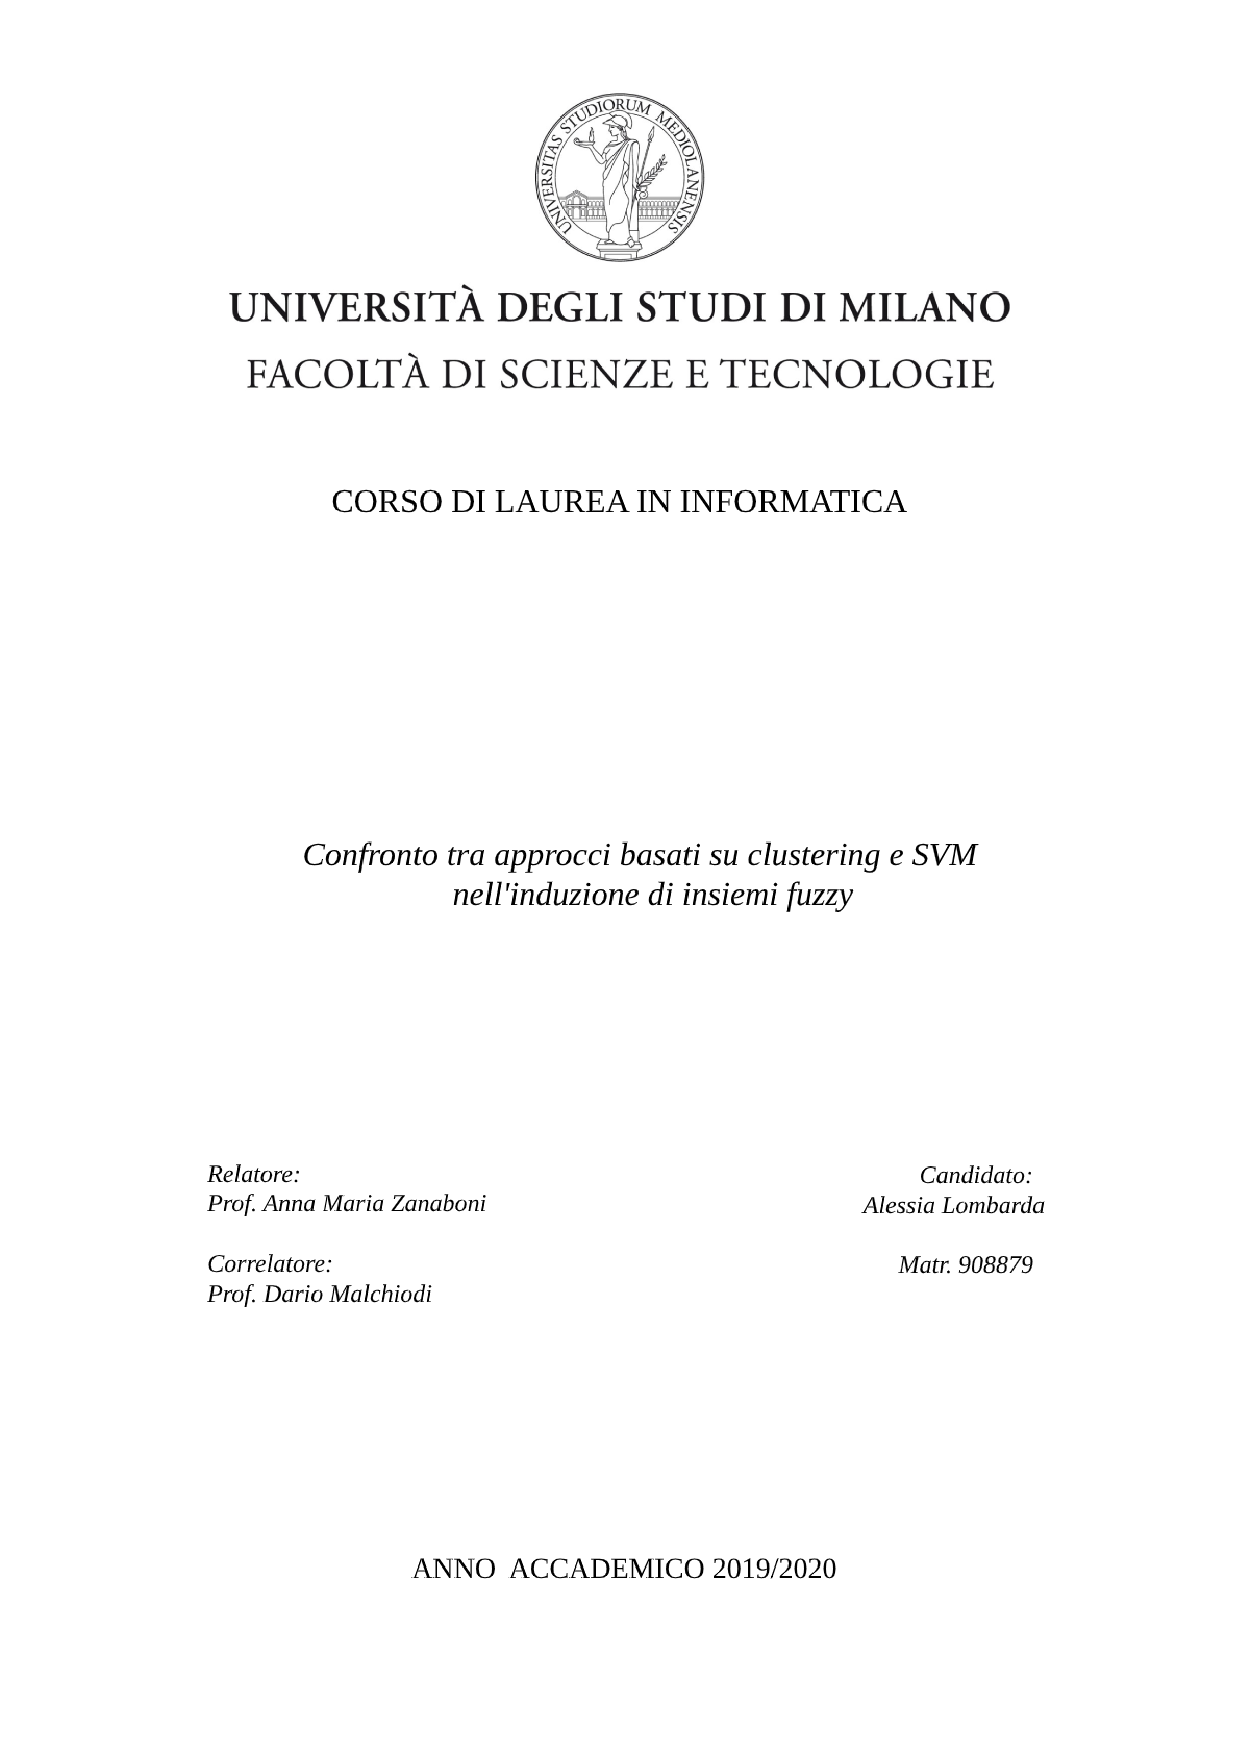
\includepdf{images/FRONTESPIZIO.pdf}
	\end{titlepage}
	\frontmatter
	\chapter*{Ringraziamenti}
	\addcontentsline{toc}{chapter}{Ringraziamenti}
	Some text...
	\tableofcontents
	\mainmatter
	%\pagenumbering{arabic}
	\chapter*{Introduzione}
		{} \addcontentsline{toc}{chapter}{Introduzione}
	\chapter{Apprendimento supervisionato e induzione di insiemi fuzzy}
		\section{Apprendimento supervisionato}
		L'apprendimento automatico è una branca dell'intelligenza artificiale che studia algoritmi che utilizzano l'esperienza per migliorare la propria performance o per fare predizioni più accurate. In questo caso l'esperienza viene rappresentata attraverso una collezione di dati resi disponibili all'analisi(si può definire ogni elemento dell'insieme di dati come \textit{esempio}). Questi dati possono essere aumentati con delle \textit{etichette} (dette anche \textit{label}) impostate manualmente oppure venire estratti direttamente dall'ambiente: gli algoritmi avranno l'obiettivo di effettuare predizioni su dati non noti, sulla base della conoscenza acquisita.
		L'apprendimento automatico si applica a svariati campi quali il riconoscimento vocale, la guida autonoma di veicoli, i motori di ricerca o la ricerca scientifica in campo medico. Alcune delle classi principali di problemi che si possono affrontare con delle tecniche di apprendimento automatico sono:
		\begin{itemize}
			\item\textbf{classificazione:} l'assegnamento di oggetti a categorie; in questo caso di solito si hanno poche classi;
			\item\textbf{regressione:} la predizione di valori reali a partire da dati non noti; in questo caso l'errore associato ad una predizione errata dipende della differenza tra il valore predetto e quello reale;
			\item\textbf{ranking:} l'ordinamento di elementi in base a un criterio definito a priori;
			\item\textbf{clustering:} il partizionamento di elementi in gruppi omogenei.
		\end{itemize}
	
		L'apprendimento automatico può essere \textit{supervisionato}, \textit{non supervisionato} o \textit{semi-supervisionato}. Nell'apprendimento non supervisionato gli esempi a disposizione nell'insieme di dati forniti sono degli oggetti non associati ad etichette; l'obiettivo dell'apprendimento è quindi quello di trovare dei raggruppamenti omogenei di tali oggetti (come nel caso del clustering) sulla base di un criterio di similarità o dissimilarità definito a priori. Nell'apprendimento semi-supervisionato, invece, si hanno solitamente a disposizione una gran quantità di dati senza etichetta e un numero ridotto di dati associati ad un'informazione (che rappresenta una quantità che si vuole predire); ciò si verifica spesso in situazioni reali in cui l’etichettatura dei dati è molto costosa e/o si dispone di un flusso costante di dati. Se ad esempio consideriamo i messaggi inappropriati in un social network come insieme di dati, possiamo notare come non ci sia modo di ottenere informazioni etichettate a mano su ogni messaggio, perché a causa della grande quantità di dati sarebbe troppo costoso. Possiamo quindi etichettare a mano un sottoinsieme di essi e, sfruttando le tecniche semi-supervisionate, utilizzare questo piccolo set di dati etichettati per comprendere il resto del contenuto dei messaggi.\newline
		Nell'apprendimento supervisionato l'informazione aggiuntiva (detta \textit{etichetta} o \textit{label}) è invece specificata per ogni dato a disposizione; lo scopo dell'algoritmo è quello di trovare un modello che permetta di effettuare predizioni anche su dati non noti.
		Si può modellare quindi una funzione $f$ che associa ad ogni dato la corrispondente etichetta; lo scopo dell'apprendimento supervisionato è quello di determinare (a partire dai dati) una funzione $h$ che approssimi in modo accettabile\footnote{definire una metrica che indichi la bontà dell'approssimazione è un problema significativo} la funzione $f$. Sia $f$ che $h$ sono funzioni di un vettore di input $X=(x_1,x_2,...,x_i,...,x_n)$ di $n$ componenti (detti anche \textit{feature})~\cite{bib:ml}.
		Nel caso di apprendimento supervisionato si conoscono quindi (a volte solo in modo approssimato) i valori di $f$ per gli $m$ elementi del training set, $\Xi$. Assumiamo che, se possiamo trovare una funzione $h$ che restituisce valori che approssimano in modo accettabile quelli di $f$ per gli elementi di $\Xi$, allora questa funzione costituisce una buona approssimazione per $f$, specialmente se $\Xi$ è grande.
		
		Per quanto riguarda il vettore di input $X$, questo può essere costituito da valori reali, discreti o categorici, che a loro volta possono essere ordinati (ad esempio \textit{\{piccolo, medio, grande\}}) o non ordinati (ad esempio \textit{\{nord, sud, est, ovest\}}); un caso a sé è costituito dall'uso di valori booleani, che può essere considerato un caso particolare dell'utilizzo di numeri discreti (1,0) o di variabili categoriche (\textit{True}, \textit{False}).\newline
		L'output della funzione può essere invece un numero reale, ovvero una stima, oppure un valore categorico, tipico dei classificatori. Nel caso di output booleani, invece, possiamo distinguere \textit{istanze positive}, ovvero quelle con label 1, e \textit{istanze negative}, quelle con label 0; se anche l'input è booleano il classificatore implementa una \textit{funzione booleana}.\\
		
		Definiamo ora il \textit{bias}, ovvero un insieme di informazioni che definisce la potenza rappresentativa di un modello di apprendimento; il termine bias venne introdotto da Mitchell(1908) a significare "ogni informazione su cui ci si basa per scegliere un'ipotesi di generalizzazione rispetto ad un altra". Si possono distinguere due tipi di bias: quello assoluto e quello relativo. Il \textit{bias assoluto} è un'assunzione fatta dall'algoritmo di apprendimento che restringe l'insieme delle possibili funzioni target(ovvero quelle tra cui scegliere la funzione $h$ che approssima $f$) a un sottoinsieme di funzioni (ad esempio le funzioni lineari, o quelle booleane).
		Il \textit{bias relativo}, invece, assume che la funzione da apprendere sarà probabilmente in un insieme di funzioni invece che in un altro~\cite{bib:bias}.
		Se ad esempio si considera un algoritmo che deve approssimare una funzione booleana in $n$ variabili, si potranno avere $2^n$ possibili input. 
		\begin{figure}[h]
			\centering
			\subfloat[\emph{}]
			{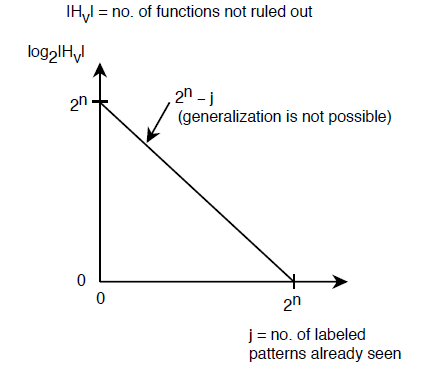
\includegraphics[width=.45\textwidth]{nobias.png}} \quad
			\subfloat[\emph{}]
			{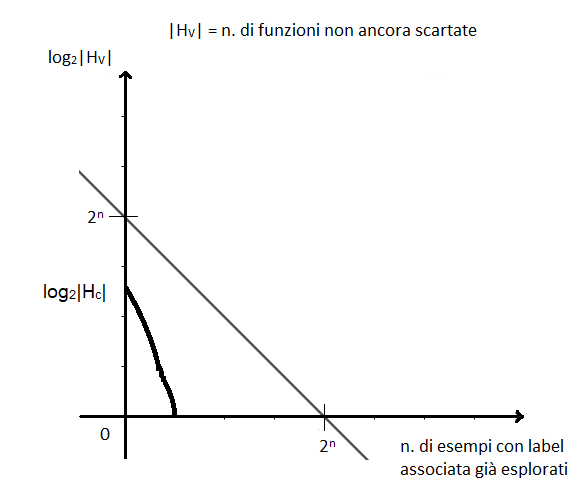
\includegraphics[width=.45\textwidth]{bias.png}} \\
			\caption{Relazione tra il numero di funzioni possibili e gli elementi del training set già esplorati in assenza e presenza di bias}
			\label{fig:bias}
			
		\end{figure}
		Si supponga di non avere bias, che si stia considerando l'insieme $\mathcal{H}$ delle $2^{2^n}$ possibili funzioni booleane e che non si abbiano preferenze tra quelle che danno corrispondenze sull'insieme dei dati usati per l'apprendimento (detto \textit{training set}). In questo caso, dopo aver considerato un elemento del training set e la sua etichetta si potrà suddividere a metà l'insieme delle funzioni, ovvero distinguere quelle che classificherebbero correttamente quell'elemento dalle restanti. Presentando via via più elementi del training set, ad ogni passo del processo si dimezza il numero di funzioni considerabili come ipotesi di approssimazione per $f$, come mostrato in Figura \ref{fig:bias}a. Non è possibile in questo caso generalizzare, perché le corrispondenze già trovate non danno alcun indizio su quelle ancora da scoprire: è solo possibile memorizzare le prime, e ciò causa un apprendimento molto oneroso.\newline
		Se invece si limitasse l'insieme $\mathcal{H}$ a un sottoinsieme $\mathcal{H}_c$, dipendentemente dal sottoinsieme e dall'ordine di presentazione dei dati del training set, la curva che rappresenta il numero di possibili ipotesi di funzioni apparirebbe come in Figura~\ref{fig:bias}b: potrebbe infatti accadere che dopo aver visto meno di $2^n$ campioni si arrivi già a selezionare una funzione $h$ che ben approssimi $f$. L'introduzione del bias, quindi, ci permette di considerare solo alcune classi di funzioni, rendendo l'apprendimento più efficiente.
		
		Spieghiamo ora il funzionamento dell'algoritmo di apprendimento: inizialmente si ha una fase di addestramento sul \textit{training set}, seguita da una fase di valutazione su un insieme distinto di dati, il \textit{test set}. Si dice che una funzione \textit{generalizza} se è in grado di predire ``bene" anche i dati presenti nel test set.\newline
		In questo contesto è anche necessario selezionare le feature da considerare per ogni campione, in quanto feature rilevanti nella soluzione del problema che si sta considerando possono guidare l'algoritmo di apprendimento correttamente, mentre altre meno rilevanti possono portare a un errore maggiore. Risulta quindi necessario, prima di procedere con l'apprendimento, utilizzare un algoritmo di \textit{feature selection}.
		
		Altra questione da considerare è la possibile presenza di rumore nei vettori del training set: possiamo distinguere il \textit{rumore di classe}, che altera il valore della funzione $f$, e quello di \textit{attributo}, che altera in modo causale i valori del vettore di input $X$; in entrambi i casi l'errore rende imprecisa la corrispondenza tra i valori di input e quelli della funzione applicata su di essi.\\
		
		Fondamentale è poi la definizione di un metodo per la valutazione della performance dell'algoritmo: consideriamo a questo scopo l'\textit{accuratezza} e le \textit{funzioni di errore}. L'accuratezza consiste nel contare il numero di predizioni corrette, e dividere questo valore per il la cardinalità del set di dati: si otterrà un valore compreso tra 0 e 1, che sarà maggiore se l'algoritmo predice in modo corretto. Un altro stimatore è l'\textit{errore quadratico medio}, che si vuole minimizzare:\\
		\[
		MSE={1\over n}\sum_{i=1}^n (y_i-h(x_i))^2\text{,}
		\]
		dove $y_i$ è la label attesa e $h(x_i)$ quella predetta dall'algoritmo, e la sua radice quadrata, l'RMSE:\\
		\[
		RMSE = \sqrt{\frac{1}{n}\sum_{i=1}^{n}(y_{i} - h(x_{i}))^{2}}\text{.}
		\]\\
		La scelta dello stimatore dipende dalla classe a cui appartiene il problema considerato: si utilizza infatti l'accuratezza nei problemi di classificazione, in cui data una label predetta possiamo dire con certezza se questa sia corretta oppure se è diversa da quella attesa; l'MSE è invece tipico dei problemi di regressione (anche se può comunque essere usato per la classificazione), in quanto considera quanto il valore reale predetto e quello atteso si discostano tra loro.
		
		Per migliorare la performance dell'algoritmo è necessario evitare che questo si specializzi eccessivamente sui dati (\textit{overfitting}). A causa della ridotta dimensione del training set disponibile, si è soliti usare una tecnica nota come \textit{n-fold cross validation}, usata sia per la model selection (la selezione dei parametri liberi dell'algoritmo), sia per la fase di valutazione della generalizzazione. Se infatti il dataset disponibile ha una dimensione ridotta, la divisione in training e test set ridurrebbe ulteriormente i dati disponibili per l'apprendimento: questo si può evitare utilizzando la cross validation, che considera nell'intero processo tutti i dati per la fase di training ma permette al contempo una fase di valutazione rigorosa, dstinguendo ogni volta dati di training e di test.\newline
		Approfondiamo inizialmente l'uso della k-fold cross validation per la fase di model selection~\cite{bib:cv}: la model selection serve per la definizione dei cosiddetti \textit{iperparametri} o \textit{parametri liberi}, ovvero parametri iniziali necessari su cui il processo di apprendimento si basa. Questi parametri sono distinti da quelli che l'algoritmo determina nel processo di apprendimento; tipici esempi sono il kernel e il parametro gamma per le Support Vector Machines.\newline
		Detto $\theta$ il vettore dei parametri liberi dell'algoritmo, ipotizziamo per semplicità che ci sia un solo parametro libero, da scegliere all'interno di un insieme di possibili valori. Per un fissato valore di $\theta$ si partiziona in modo causale un training $S$ di $m$ elementi con etichette associate in $n$ sottogruppi (\textit{fold}). L'$i$-esimo fold $S_i$ sarà quindi un campione $((x_{1}, y_{1}),...,(x_{m_i},y_{m_i}))$ di cardinalità $m_i$. Poi, per ogni $i\in\{1, ..., k\}$ l'algoritmo viene addestrato su un \textit{validation set} costituito da tutti i fold tranne l'i-esimo, per generare l'ipotesi $h_i$, e la performance di $h_i$ viene valutata sull'i-esimo fold. Il valore del parametro $\theta$ è scelto sulla base dell'errore medio di $h_i$, chiamato \textit{cross-validation error}, denotato da $\widehat{R}_{CV}(\theta)$ e definito da
		\[
		\widehat{R}_{CV}(\theta)={1\over k}\sum_{i=1}^n {1\over m_i}\sum_{(x,y)\in S_i} L(h_i(x),y)
		\]
		I fold sono generalmente definiti della stessa taglia, ovvero $m_i=m/n$ per ogni $i\in[1,n]$. La scelta di n è molto importante ai fini dell'utilizzo di questo metodo: con un $n$ grande ogni fold avrà taglia prossima ad $m$, la cardinalità dell'intero dataset, ma i fold saranno piuttosto simili, e quindi il metodo avrà un bias ridotto ed una grande varianza. Viceversa, valori bassi di $n$ portano a training set differenziati, ma la loro taglia è significativamente più bassa di $m$ e quindi il metodo tenderà ad avere una varianza minore ma un bias maggiore. I valori che generalmente si scelgono come $n$ sono 5 o 10.\newline
		\begin{figure}
			\begin{center}
				\begin{minipage}{0.47\textwidth}
					\centering
					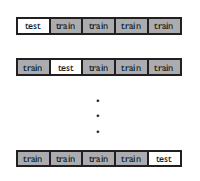
\includegraphics[width=\textwidth]{CV1.png}
					\caption{n-fold cross validation}
					\label{fig:crossval}
				\end{minipage}
				
			\end{center}
		\end{figure}
		Per la model selection, quindi, la cross validation è utilizzata in questo modo: l'intero dataset viene suddiviso inizialmente in training e test set, dove il training set ha taglia $m$. Questo viene poi utilizzato per computare il cross validation error $\widehat{R}_{CV}(\theta)$ per un certo numero di possibili valori di $\theta$; viene considerato come $\theta_0$ il valore per cui $\widehat{R}_{CV}(\theta)$ è minimo, e l'algoritmo viene addestrato con i parametri di $\theta_0$ sull'intero training set di taglia $m$. La sua performance è poi valutata sul test set.
		Il metodo si può applicare allo stesso modo per quanto riguarda la valutazione della performance: si otterranno delle valutazioni parziali (accuratezze o errori), di cui possiamo calcolare la media per avere un'indicazione della bontà dell'apprendimento. Se vogliamo svolgere al contempo una cross validation che valuti la performance e una prima fase di model selection, sarà necessario utilizzare due cross validation annidate: la cross validation esterna suddivide ogni volta i dati in training set e test set, e valuta la bontà dell'apprendimento; la cross validation interna, invece, svolge la model selection, suddividendo a sua volta il training set iniziale in fold e valutando gli iperparametri scelti di volta in volta.
		
		\section{Insiemi e logica fuzzy}
		La teoria classica degli insiemi, inizialmente formulata da Zadeh~\cite{bib:zadeh}, è basata sul concetto fondamentale di \textit{insieme} di cui un elemento fa parte oppure no, una distinzione netta che permette di identificare un chiaro confine tra ciò che appartiene e non appartiene all'insieme. Molti problemi reali non possono però essere descritti e gestiti dalla teoria classica degli insiemi, in quanto trattano elementi che hanno appartenenza solo parziale ad un dato insieme. La teoria dei \textit{fuzzy set} (o insiemi sfocati), generalizza ed estende in questo senso la teoria classica degli insiemi~\cite{bib:fuzzy, bib:fuzzy2}.\newline
		Nella teoria classica possiamo definire la funzione caratteristica di un insieme, ovvero la funzione di appartenenza a un insieme $A$ come
		\[
		X_A(x)=
		\begin{cases}
		1, & se $ x $ \in $ A$\\
		0, & se $ x $ \notin $ A$
		\end{cases}
		\]
		Ma se un elemento ha membership soltanto parziale ad un insieme dobbiamo generalizzare questa funzione per determinare il grado di membership dell'elemento stesso: un valore maggiore indicherà un grado di membership più alto all'insieme. Se consideriamo ad esempio l'insieme universo $S$ di tutti gli esseri umani, e $S_f$ come
		\[
		S_f=\Set{s \in S | s \text{ è vecchio}}\text{,}
		\]
		$S_f$ è un \textit{sottoinsieme fuzzy} di S, perché la proprietà ``vecchio'' non è ben definita e non può essere misurata in modo preciso: dobbiamo quindi stabilire una funzione che assegni il ``valore di vecchiaia" di un essere umano, ma non esiste un criterio unico o universale per scegliere questa funzione.\newline
		Un sottoinsieme fuzzy è quindi definito da un sottoinsieme e da una funzione di membership $\mu$ ad esso associata, che associa ad ogni elemento dell'insieme un valore reale nell'intervallo $[0,1]$ (si vedano alcuni esempi in Figura \ref{fig:membership}).\\
	
		\begin{figure}[h]
			\centering
			{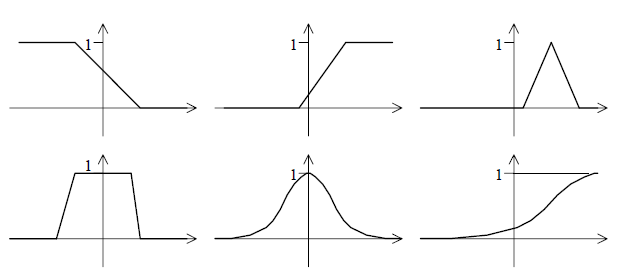
\includegraphics[width=.90\textwidth]{membership.png}} \quad
			\caption{Forme di funzioni di membership comunemente usate}
			\label{fig:membership}
			
		\end{figure}
	
		La definizione di insiemi fuzzy ha come base la logica fuzzy, che estende e potenzia la logica classica. La logica classica, infatti, riguarda proposizioni che possono essere vere o false ma che non possono mai assumere contemporaneamente entrambi i valori di verità, che hanno opposto e possono essere combinate tra loro.
		La logica fuzzy, che pone la base del ragionamento approssimato, si differenzia da quella classica in quanto ammette l'utilizzo termini linguistici imprecisi come
		\begin{itemize}
			\item{\textit{predicati fuzzy}}: vecchio, giovane, alto, veloce,
			\item{\textit{quantificatori fuzzy}}: molto, poco, quasi, di solito,
			\item{\textit{valori di verità fuzzy}}: molto vero, probabilmente falso, sicuramente falso,
		\end{itemize}	
		che permettono di trattare fenomeni della realtà difficilmente descrivibili in modo quantitativo utilizzando la logica classica, ma su cui la maggior parte del ragionamento umano si basa.
		In particolare si dicono \textit{variabili linguistiche} gli attributi dei sistemi fuzzy che assumono \textit{valori linguistici} espressi in linguaggio naturale. Questi valori hanno un significato e non un preciso valore numerico, e partizionano i possibili valori delle variabili linguistiche in modo soggettivo (ovvero solitamente basato sull'intuizione umana).
		Se ad esempio consideriamo come variabile linguistica la superficie abitabile $A$ di un appartamento, e definiamo i valori linguistici $\{molto\text{ }piccolo, piccolo, medio, grande, molto\text{ }grande\}$ e le funzione di membership $\mu_{k}$, con $k={mp, p, m, g, mg}$ (in corrispondenza dei termini linguistici), descritte come in Figura \ref{fig:mem2}, possiamo notare che ogni $x \in A$ ha $\mu(x) \in [0,1]$ per ogni valore. Se ad esempio consideriamo $x=41m^2$, avremo che $\mu_{mp}(x)=\mu_p(x)=\mu_{mg}(x)=0$, mentre $\mu_m(x)=0.1$ e $\mu_m(x)=0.9$.
		
		
		\begin{figure}[h]
			\centering
			{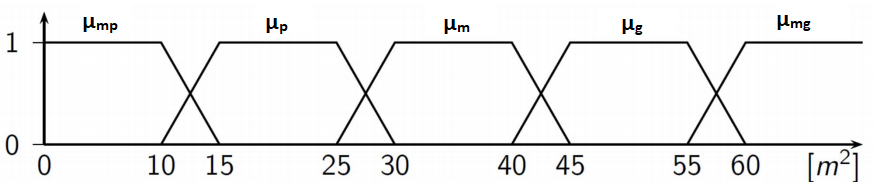
\includegraphics[width=.80\textwidth]{mem2.png}} \quad
			\caption{Esempio: funzioni di membership in riferimento alla superficie abitabile di un appartamento}
			\label{fig:mem2}
		\end{figure}
		 
		L'applicazione della logica fuzzy a problemi di apprendimento passa attraverso l'utilizzo dei \textit{FIS} (Fuzzy Inference Systems), che sono composti da cinque blocchi funzionali(Figura \ref{fig:fis}): 
		\begin{itemize}
			\item{\textit{rule base}}: contiene le regole if-then fuzzy definite da esperti,
			\item{\textit{database}}: definisce le membership function dei fuzzy set usati nelle regole fuzzy,
			\item{\textit{inference engine}}: esegue operazioni sulle regole,
			\item{\textit{fuzzifier}}: converte le quantità crisp (ovvero valori numerici trattabili dalla logica classica) in quantità fuzzy,
			\item{\textit{defuzzifier}}: converte le quantità fuzzy in quantità crisp.
		\end{itemize}
		\begin{figure}[h]
			\centering
			{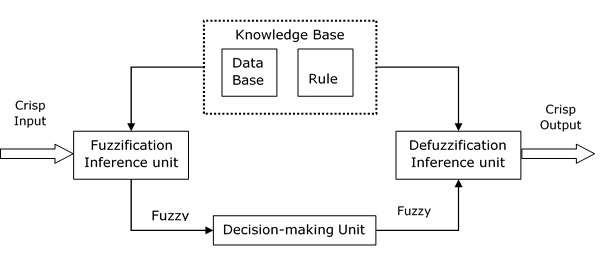
\includegraphics[width=.80\textwidth]{fis.jpg}} \quad
			\caption{Struttura di un FIS}
			\label{fig:fis}
		\end{figure}
	
		Il FIS quindi, e in particolare il fuzzifier converte l'input da crisp a fuzzy, aggiornando la Knowledge Base formata da Database e Rule base; l'input viene poi passato all'Inference Engine, che determina il match con le regole if-then (e aggiorna le regole stesse sulla base dell'input), ovvero associa input fuzzy ad output fuzzy, che viene poi ritrasformato in output crisp dal defuzzifier.

		I concetti della teoria degli insiemi fuzzy applicati all'apprendimento automatico hanno portato alla nascita del \textit{fuzzy machine learning}, che ha permesso l'estensione di tecniche di apprendimento non fuzzy a corrispondenti tecniche fuzzy: si può parlare di fuzzy clustering, fuzzy support vector machines, fuzzy k-nearest neighbour e così via. Queste tecniche sono utilizzate principalmente in tre ambiti: quelli di classificazione e data analysis, i problemi di decision-making e il ragionamento approssimato; questi problemi mostrano le tre semantiche attribuibili al grado di membership, ovvero la similarità, la preferenza e la possibilità.\newline
		Per quanto riguarda la prima categoria, che approfondiremo in seguito, il grado di membership $\mu(u)$ di un elemento $u$  indica la relazione tra oggetti di un universo, in termini di similarità, dissimilarità o in funzione della distanza; questa semantica è specialmente utilizzata per problemi di classificazione, clustering e regressione. Per quanto riguarda invece la preferenza, dato un insieme di oggetti e una funzione di membership quest'ultima rappresenta quanto si favorisce un determinato oggetto rispetto agli altri; interpretando la funzione di membership come grado di incertezza, infine, si intende il valore della funzione di membership $\mu$ come il grado di possibilità che un oggetto $x$ abbia valore $u$~\cite{bib:dubois}.
		
		Nel campo dell'apprendimento automatico, quindi, le tecniche di induzione di funzioni di appartenenza producono modelli che trasformano variabili di input in gradi di appartenenza ad un insieme fuzzy. Si possono distinguere a questo proposito tecniche induttive o deduttive: l'uso di metodi deduttivi implica la definizione di funzioni di appartenenza da parte di esperti, ovvero sulla percezione umana (tecniche \textit{data-driven}). Le tecniche induttive, invece, prevedono la generazione delle funzioni di appartenenza sulla base dei dati (tecniche \textit{data-driven}). Si approfondiranno in seguito queste ultime, più affidabili in quanto slegate dalle diverse interpretazioni che esperti possono dare agli stessi attributi o variabili.
	
		\chapter{Tecniche per induzione della funzione di membership}
		Ottenere la funzione di membership a partire dai dati di training è uno dei problemi fondamentali legati all'applicazione della teoria dei fuzzy set, in cui le funzioni di membership vengono utilizzate per mappare l'imprecisione dell'informazione in input. Non ci sono però regole o linee guida che possano essere usate per scegliere l'appropriata tecnica di generazione, e il problema è reso più complesso dalla mancanza di accordo sulla definizione e interpretazione delle funzioni di membership. Le diverse tecniche di induzione spaziano da tecniche basate sulla percezione, ovvero sul giudizio umano o di esperti, a tecniche euristiche, che usano forme di funzioni di membership predefinite, tecniche basate su istogrammi (che utilizzano appunto istogrammi per considerare la distribuzione delle features di input), trasformazione di distribuzioni di probabilità in distribuzioni di possibilità, tecniche basate su fuzzy nearest neighbour o su reti neurali (come approfondito in ~\cite{bib:rita}), su clustering o support vector machines (che approfondiremo meglio in seguito); l'intera rassegna è presentata in~\cite{bib:rassegna}.
		
		\section{Clustering}
		Gli algoritmi classici di clustering hanno come fine il raggruppamento e la selezione di elementi omogenei in un insieme di dati. Dati in input $n$ oggetti, l'algoritmo restituisce in output un clustering $\mathcal{C}=\{c_1, ..., c_k\}$ degli oggetti, ovvero una partizione dell'insieme degli elementi $V$. Due elementi sono detti omogenei o disomogenei in relazione ad una funzione di similarità o dissimilarità $\sigma: V\times V\rightarrow \mathbb{R}$, detta \textit{metrica}, che assegna un valore ad ogni possibile coppia di punti: un esempio banale può essere costituito da una funzione che assegna il valore $1$ ad elementi omogenei e il valore $-1$ ad elementi disomogenei. Si possono utilizzare svariati tipi di funzioni: un esempio comune è la norma (distanza euclidea, una funzione di dissimilarità), che dati due punti $u$ e $v$ è definita come:
		\[
			\sigma(u, v) = \norma{u - v}\text{.}
		\]
		
		\subsection{Breve classificazione}
			Dati $v$ e $\sigma$, posso operare due diversi tipi di clustering: il clustering \textit{partition based}, che utilizza una distanza da un punto rappresentativo del cluster (ad esempio il \textit{centroide}) per determinare l'appartenenza di un elemento ad un gruppo, avendo prefissato il numero di gruppi della partizione risultato, oppure clustering \textit{gerarchico}, in cui viene costruita una gerarchia di partizioni visualizzabile mediante una rappresentazione ad albero (dendrogramma), in cui sono rappresentati i passi di accorpamento/divisione dei gruppi stessi.\\
			Le tecniche di clustering si possono inoltre suddividere sulla base del modo in cui operano in \textit{metodi aggregativi} (o \textit{bottom-up}) e \textit{metodi divisivi} (o \textit{top-down}). La prima classe comprende i metodi che considerano inizialmente tutti gli elementi come cluster a sé, e in cui poi l'algoritmo provvede ad unire i cluster più vicini. L'algoritmo continua questo processo fino ad ottenere un numero prefissato di cluster, oppure fino a che la distanza minima tra i cluster non supera un certo valore, o ancora in relazione ad un determinato criterio statistico prefissato.
			I metodi divisivi, invece, prevedono che all'inizio tutti gli elementi siano in un unico cluster: l'algoritmo, poi, inizia a dividere il cluster in tanti sottoinsiemi di dimensioni inferiori, cercando di ottenere gruppi sempre più omogenei. L'algoritmo procede fino a che non viene soddisfatta una regola di arresto, che è generalmente legata al raggiungimento di un numero prefissato di cluster.\\
			\`E possibile inoltre operare un'ulteriore classificazione delle tecniche di clustering: si distingue il clustering di tipo \textit{esclusivo} o \textit{hard clustering}, in cui ogni elemento può essere assegnato ad uno e ad un solo gruppo (di conseguenza i cluster saranno a due a due disgiunti) e il clustering \textit{non-esclusivo}, noto anche con il nome di \textit{soft clustering} o \textit{fuzzy clustering}.

	\subsection{Fuzzy clustering}
		I problemi di clustering possono avere applicazioni in svariati campi, come l'economia, psicologia, medicina, biologia; ne è fatto in particolare un vasto utilizzo nel campo della bioinformatica, in cui il fuzzy clustering è preferito a quello classico, nel campo del marketing, in cui ad esempio gli utenti possono essere suddivisi in cluster fuzzy sulla base di bisogni, preferenze e profili o ancora nell'image analysis, in cui è usato in particolare per la segmentazione al fine di svolgere pattern recognition, object detection, e analisi di immagini mediche.
		Nel fuzzy clustering infatti, in opposizione alle tecniche classiche di clustering come il \textit{k-means}, gli elementi di input possono appartenere a più di una partizione, con un certo valore di membership. La membership non rappresenta però una probabilità: la somma dei valori di membership assegnati ad un elemento in relazione a classi opposte non deve perciò dare 1; la membership sarà più bassa se il punto si colloca sul limite esterno del cluster, e viceversa maggiore se l'elemento è vicino al centro del cluster.
		
		La maggior parte dei metodi di fuzzy clustering esistenti fa riferimento come base al \textit{Fuzzy C-Means}, la variante fuzzy del classico k-means. L'algoritmo \textit{k-means}, proposto nel 1967 da MacQueen, è uno degli algoritmi di apprendimento base utilizzato per risolvere problemi di clustering; lo scopo è quello di classificare un dataset di cardinalità $n$ in un certo numero di cluster $k$, definito a priori.
		Si definiscono inizialmente $k$ \textit{centroidi}, uno per ogni cluster, a rappresentare i centri inziali del cluster stesso. Questi centroidi devono essere scelti in modo accurato, e preferibilmente inizialmente distanti gli uni dagli altri: la posizione dei centroidi iniziali influisce infatti sul risultato del clustering. Successivamente, si assegna ogni punto nel dataset al centroide ad esso più vicino (utilizzo come funzione di similarità la norma); a questo punto si ricalcolano i $k$ nuovi centroidi, ottenuti come baricentro dei punti in un dato cluster. Si ripetono queste due operazioni di riassegnazione dei punti e correzione dei centroidi finchè non si hanno più cambiamenti significativi, ovvero finchè il clustering è stabile. Lo scopo di questo algoritmo è infatti quello di minimizzare una funzione obiettivo $J$, espressa come
		\[
			J = \sum_{j=1}^{k}\sum_{i=1}^{n}\norma{x_i^{(j)}-c_j}^2\text{,}
		\]
		ovvero la somma dei quadrati delle distanze di ogni punto dal centro del cluster a cui appartiene. 
		L'algoritmo k-means termina sempre, ma non trova necessariamente il clustering ottimo (quello che minimizza la funzione obiettivo): il problema infatti è np-hard, e l'algoritmo è molto sensibile alla posizione dei cluster iniziali. Per ridurre questo effetto è necessario ripetere più volte l'esecuzione dell'algoritmo.\\
		
		Il \textit{Fuzzy C-Means} parte quindi da questa base e generalizza l'algoritmo in senso fuzzy: in questo algoritmo, gli oggetti che si collocano sul confine di un dato cluster non sono forzati ad appartenere ad un solo cluster, ma possono invece appartenere a diversi insiemi con una membership parziale compresa tra 0 e 1, garantendo una prestazione migliore specialmente in presenza di rumore nei dati o outliers~\cite{bib:kmvsfcm}. 
		Gli elementi saranno quindi assegnati ad ogni cluster con diversi valori di appartenenza: punti più vicini al centro del cluster avranno membership maggiore, e viceversa punti lontani avranno membership minore.\\
		Fissato un dato numero di cluster $c$, dove $2\leq c \le n$,  e selezionato un valore per il parametro $m$ (che controlla la fuzziness e approfondiremo in seguito), è necessario quindi inizializzare la partition matrix $U$. La matrice $U=[u_{ik}]$ è una matrice $c\times N$ di numeri reali, dove $u_i$  è la funzione caratteristica dell'insieme che mappa i valori di membership degli $y_k$ nel sottoinsieme fuzzy di $Y$, dove $0\leq u_{ic}\leq 1$
		e $y_k$ è il k-esimo feature vector, e
	
		\[
		\sum_{j=1}^{N}u_{ik} > 0\text{ } \forall i\\
		\]
		\[
		\sum_{j=1}^{N}u_{ik} = 1 \text{ }\forall k\text{.}
		\]
		
		Si possono scegliere varie funzioni come metriche per misurare la similarità; la più nota è l'uso dei \textit{minimi quadrati generalizzati} (o Generalized Least Squares, GLS), definita come
		\[
			J_m(U, v)=\sum_{k=1}^{N}\sum_{i=1}^{c}u_{ik}^m\norma{y_k-v_i}^2_A\text{,}
		\]
		dove:
		\begin{itemize}
			\item $Y = {y_1, y_2, ..., y_N} \subset \mathbb{R}^n$ è l'insieme dei dati, 
			\item $2 \leq c < n$ è il numero di cluster desiderati,
			\item $1 \leq m <\infty$ è il parametro che esprime la fuzziness,
			\item $U$ è la partizione fuzzy di $Y$,
			\item $v = (v_1, v_2, ..., v_c)$ è il vettore dei centri,
			\item $v_i = (v_{i1}, v_{i2}, ..., v_{in})$ è il centro del cluster $i$,
			\item $\norma{\textit{ }}_A$ è la norma indotta su $\mathbb{R}^n$,
			\item $A$ è una matrice positiva di pesi $n\times n$,
		\end{itemize}
		e la distanza quadratica tra $y_k$ e $v_i$ nella formula è calcolata come
		\[
			d^2_{ik} = \norma{y_k-v_i}^2_A = (y_k-v_i)^TA(y_k-v_i)\text{.}
		\] 	
		Ogni errore quadratico è poi pesato con $(u_{ik})^m$, l'm-esima potenza della membership degli elementi $y_k$ nel cluster $i$.\\
		Sono necessarie a questo punto delle considerazioni sui parametri $m$ ed $A$. Si può infatti notare che per $m\rightarrow 1$ il clustering diventa più netto e con $m=1$ si ottiene un hard clustering. Solitamente si utilizzano $m \in\{1,2,...,30\}$, anche se per la maggior parte dei dati un valore di m compreso tra 1.5 e 3.0 dà buoni risultati. \\
		Per quanto riguarda invece la matrice $A$, questa controlla la forma che i cluster di $Y$ assumeranno; si possono usare a questo proposito diversi tipi di norme.
		
		Un clustering fuzzy ottimale è dunque definito da una coppia $(U, v)$ che minimizza $J_m$; possiamo descrivere quindi l'algoritmo FCM come segue.
		Definita con $r=0,1, ...$ ogni interazione dell'algoritmo, e fissati $c$, $m$, $A$ e $\norma{k}_A$, si definisce la matrice iniziale $U^{(0)}$. Successivamente è necessario calcolare ad ogni passo il vettore dei $c$ centri, e poi una membership matrix aggiornata $U^{(k+1)}$. Si itera l'esecuzione dell'algoritmo finchè l'errore commesso nell'assegnamento delle membership (ovvero la norma calcolata sulla differenza tra la matrice delle membership calcolata al tempo k e k+1) non scende sotto una soglia $\epsilon$~\cite{bib:fcm}.
		
		Il Fuzzy C-Means si può quindi considerare l'algoritmo alla base del fuzzy clustering; a partire da questo si sono poi sviluppate una serie di varianti che trattano diverse forme di funzioni di appartenenza, che pongono un'attenzione particolare al rumore e agli outliers come RSFKM~\cite{bib:rsfkm} e GEPFCM~\cite{bib:gifpfcm}, algoritmi che risolvono il problema di stabilire a priori il numero di cluster e la sensibilità di FCM alla posizione dei centroidi iniziali, come in~\cite{bib:afkm} o ancora che utilizzano come funzioni di similarità tecniche diverse dalla distanza euclidea, come in KFCM~\cite{bib:kfcm}.
		\\
		Oltre a questa categoria di algoritmi si distinguono algoritmi di fuzzy support vector clustering, una tecnica ibrida tra clustering e uso di support vector machines (come in~\cite{bib:svc,bib:msvc}).
		\\
		Una rassegna completa dei vari tipi di algoritmi è disponibile in Tabella \ref{tab:clustering}
		\begin{table}[h!]
			\caption{Rassegna di metodi per fuzzy clustering}
			\begin{center}\begin{tabular}{ |c|c|c|c| } 
					\hline
					Categoria & Nome metodo & Anno di pubblicazione & Articolo\\
					\hline
					\multirow{10}{4em}{estensioni a FCM} 
					& RSFKM & 2016 & \cite{bib:rsfkm}\\ 
					& Agglomerative FCM & 2008 & \cite{bib:afkm}\\
					& FKM con FIS & 2013 & \cite{bib:fkmfis}\\ 
					& GIFP-FCM & 2009 & \cite{bib:gifpfcm}\\
					& BCPFCM, BCPNFCM e BCSP NFCM & 2016 & \cite{bib:bcpfcm}\\
					& REFCMFS & 2019 & \cite{bib:refcmfs}\\ 
					& CSFCM & 2015 & \cite{bib:csfcm}\\
					& ICFFCM & 2019 &\cite{bib:icffcm}\\
					& KFCM & 2003 &\cite{bib:kfcm}\\
					& DOFCM & 2011 & \cite{bib:dofcm}\\
					\hline													
					\multirow{2}{4em}{Support Vector Clustering}	& SVC & 2013 & \cite{bib:svc}\\ 
					& MSVC & 2016 & \cite{bib:msvc}\\ 
					&  &  & \\
					\hline
					& Shadowed Set Induction & 2018 & \cite{bib:ssi} \\
					\hline
					\multirow{2}{4em}{Spectral Clustering}	& FKSC & 2018 & \cite{bib:fksc}\\ 
					& SSC-PC & 2016 & \cite{bib:sscpc}\\ 
					\hline
					& PFCM & 1993 & \cite{bib:pfcm}\\
					\hline
				\end{tabular}
			\end{center}
			\label{tab:clustering}	
		\end{table}
	
	\section{Support Vector Machines}
	Le \textit{Support Vector Machines}, sviluppate da Vapnik nel 1995, sono una tecnica di apprendimento supervisionato utilizzato soprattutto per problemi di classificazione, regressione e detection di outliers; esse sono utilizzate per un vasto numero di applicazioni, dal riconoscimento facciale al processing di dati biologici per diagnosi mediche.
	
	Le SVM hanno come obiettivo quello di identificare un iperpiano ``ottimo" come soluzione del problema di apprendimento, ovvero un iperpiano che distingua diverse classi di elementi dell'insieme dei dati di input e che massimizzi il \textit{margine}, ovvero la massima distanza tra i punti delle classi più vicini all'iperpiano e l'iperpiano stesso. In uno spazio bidimensionale, un iperpiano è quindi una retta che divide il piano in due semizpazi. La formulazione più semplice delle SVM è quella lineare, in cui l'iperpiano giace sullo spazio dei dati di input $x$. Lo spazio d'ipotesi sarà quindi in questo caso un sottoinsieme dell'insieme che contiene tutti gli iperpriani della forma 
	\[
	f(x) = w\cdot x+b\text{.}
	\]
	Se i dati non sono linearmente separabili (come in Figura \ref{fig:hyp}a), però, potrebbe accadere che questo iperpiano non sia identificabile: la soluzione è quella di aggiungere un'ulteriore dimensione ottenuta come combinazione delle precedenti (trasformazione indotta da un kernel, Figura \ref{fig:hyp}b), in modo da ottenere un ulteriore spazio a più dimensioni, detto \textit{spazio delle features}, e identificare nel nuovo spazio un iperpiano ottimo (Figura \ref{fig:hyp}c).\\
		\begin{figure}[h]
		\centering
		\subfloat[\emph{}]
		{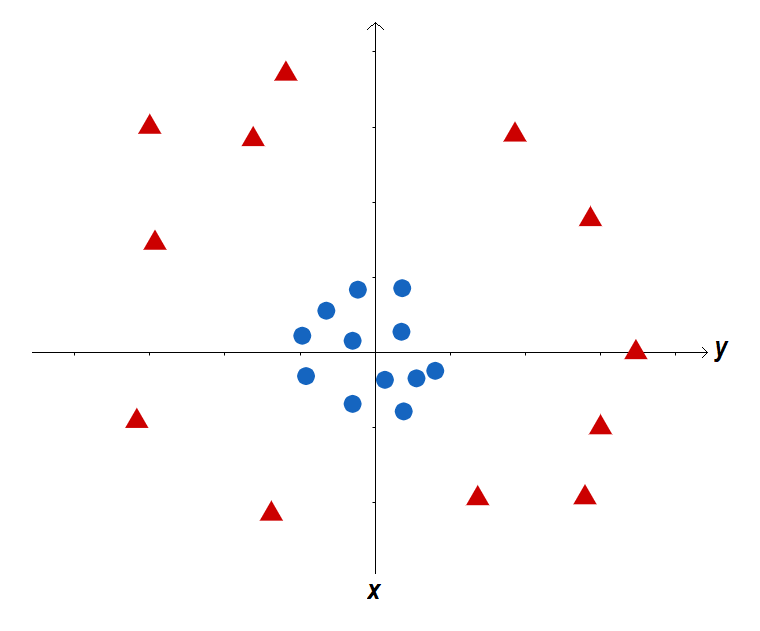
\includegraphics[width=.48\textwidth]{svm2d.png}} \quad
		\subfloat[\emph{}]
		{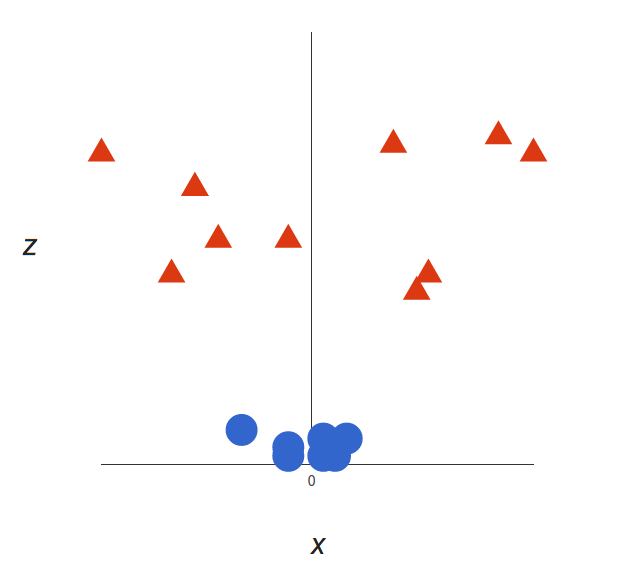
\includegraphics[width=.48\textwidth]{svm3d.png}} \quad
		\subfloat[\emph{}]
		{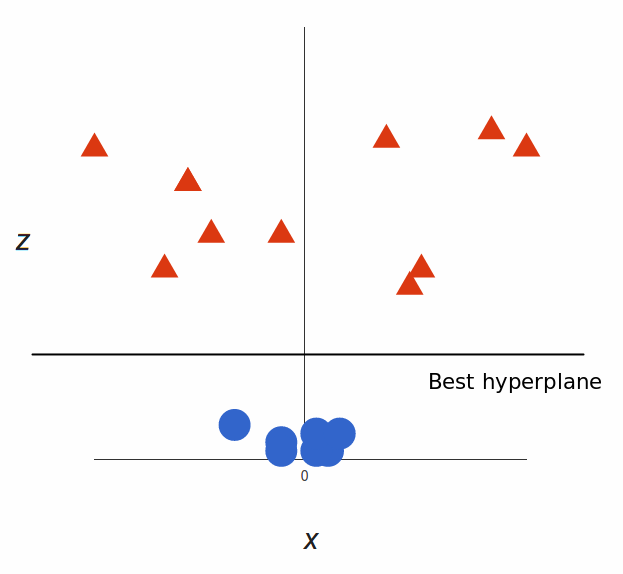
\includegraphics[width=.48\textwidth]{svm3dhyp.png}} \quad
		\subfloat[\emph{}]
		{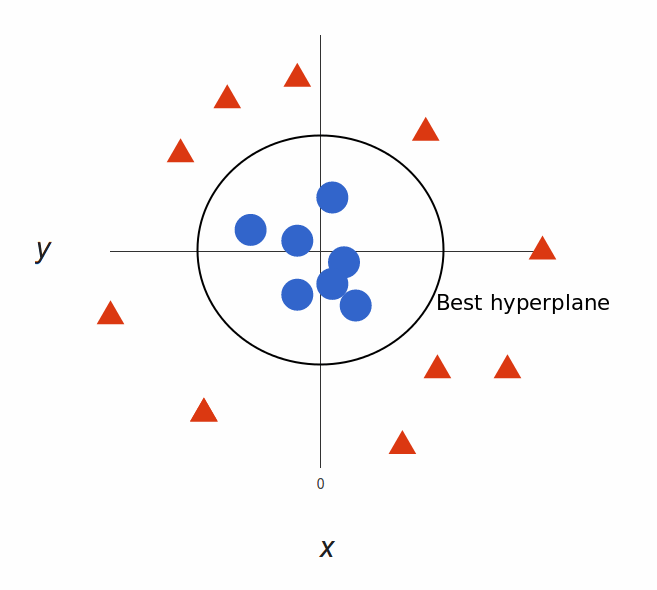
\includegraphics[width=.48\textwidth]{svm3dto2d.png}} \quad
		\caption{Passaggio allo spazio delle features in caso di dati non linearmente separabili}
		\label{fig:hyp}
	\end{figure}	
	L'uso delle SVM prevede inoltre una fase di tuning dei parametri, che in questo caso sono il \textit{kernel}, il \textit{parametro di regolarizzazione} e \textit{gamma}. Per quanto riguarda il \textit{kernel}, questo stabilisce il tipo di trasformazione che lo spazio iniziale subisce: si distinguono ad esempio kernel lineari, polinomiali ed esponenziali (questi ultimi due calcolano l'iperpiano separatore in uno spazio a più dimensioni). Il \textit{parametro di regolarizzazione}, invece, esprime quanto è importante che ogni punto venga classificato in modo corretto: per valori grandi, l'algoritmo sceglierà un iperpiano con un margine minore, affinché tutti i punti vengano assegnati alla classe corretta; viceversa per valori bassi del parametro l'iperpiano avrà margine maggiore, ma alcuni punti saranno classificati in modo non corretto, come si può vedere in \ref{fig:svm}.
	
	\begin{figure}[h]
		\centering
		\subfloat[\emph{}]
		{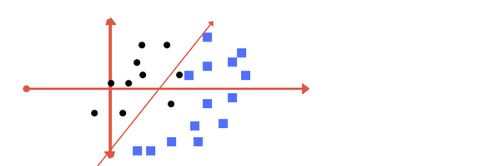
\includegraphics[width=.45\textwidth]{svm.png}} \quad
		\subfloat[\emph{}]
		{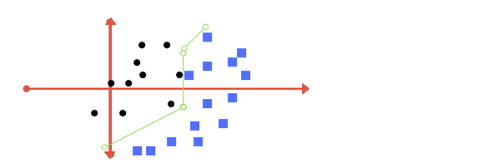
\includegraphics[width=.45\textwidth]{svm2.png}} \\
		\caption{Sulla destra: valori bassi del parametro di regolarizzazione; sulla sinistra valori più elevati}
		\label{fig:svm}
	\end{figure}
	Il parametro \textit{gamma}, infine, indica quanto lontano dall'iperpiano arriva l'influenza del singolo punto, dove valori bassi del parametro indicano che punti lontani dal possibile iperpiano influenzano la scelta dell'iperpiano stesso, e viceversa.	
	
	\section{Fuzzy Support Vector Machines}
	Le \textit{Fuzzy Support Vector Machines} estendono il concetto di SVM, generalizzandolo e applicandolo alla logica fuzzy. Nelle FSVM, infatti, l'importanza di ogni elemento del training set alla determinazione della superficie separatrice è differente: ad ogni punto è infatti assegnato un grado di membership fuzzy, che denota il contributo fornito dal punto all'apprendimento dell'iperpiano separatore. Se ad esempio un punto viene identificato come outlier, ad esso verrà assegnato un valore di membership basso, in modo che il suo contributo all'errore complessivo sia poco rilevante. Supponiamo che i dati di training siano definiti da $S = \{(x_i, y_i, s_i)| i=1,2,...,l\}$, dove ogni $x_i \in \mathbb{R}^d$ è un elemento del training set, $y_i \in \{+1, -1\}$ è la label ad esso associata e $s_i(i=1,2,...,l)$ è una membership fuzzy $r \leq s_i \leq 1$ ($r$ è una costante dal valore molto basso ma maggiore di zero). Definiamo $Q=\{x_i|(x_i, y_i, s_i)\in S\}$; possiamo partizionare in $Q$ due sottoinsiemi: la classe $C^+$, ovvero la classe dei punti a cui è associata label $y_i=+1$, e quella $Q^-$, che conterrà gli $x_i$ tali che $y_i=-1$. Il problema di classificazione può quindi essere descritto come segue:
		\[
		min \frac{1}{2} \norma{w}^2+C\sum_{i=1}^{l}s_i\xi_i
		\]
		\[	
		\text{t.c. } y_i(w^T\cdot \Phi(x_i)+b)\geq 1-\xi_i \text{, } i=1, 2, ..., l
		\]
		\[
		\text{e } \xi_i \geq 0\text{,}		
		\]
	
	dove $C$ è un valore che definisce il costo della violazione del vincolo, $\xi_i$ è una misura dell'errore nella FSVM e quindi il termine $si\xi_i$ è una misura pesata dell'errore~\cite{bib:fsvm,bib:fsvm2}.\\
	
	A partire dal metodo base delle FSVM si sono sviluppate varianti che mirano ad ottimizzarlo e adattarsi alle diverse situazioni: sono state introdotte ad esempio nuove funzioni di membership, algoritmi di ottimizzazione come in~\cite{bib:firefly}, che sfrutta l'algoritmo Firefly. Altri algoritmi si sono invece specializzati in problemi multiclasse~\cite{bib:multi}, o ancora sono stati ottimizzati per dataset con rumore nei dati o outliers, come in ~\cite{bib:apso,bib:wcs}. Una rassegna più esaustiva è mostrata in Tabella \ref{tab:svm}.
	
	Consiederiamo in particolare le Fuzzy Support Vector Machines per il \textit{Class Imbalance Learning}~\cite{bib:cil}: questo algoritmo si specializza su apprendimento in caso di dataset con rappresentanze differenti delle due classi in considerazione, in cui cioè si hanno molti meno esempi appartenenti a una classe rispetto a quelli appartenenti ad un'altra. In questo caso, con algoritmi tradizionali può accadere che l'apprendimento dia risultati molto accurati sulla predizione della classe maggiormente rappresentata, ma che commetta molti errori sull'altra classe (consideriamo ad esempio quella positiva come classe di minoranza, come nella maggior parte dei dataset reali).\newline
	Tra i metodi CIL, ovvero quelli che si occupano di questo tipo di probelma, si possono distinguere metodi interni ed esterni: i \textit{metodi esterni} fanno un preprocessing dei dati in modo da bilanciarli, ad esempio eliminando in modo casuale degli elementi della classe più rappresentata finchè un determinato rapporto tra il numero degli elementi in ogni classe viene raggiunto; un altro metodo esterno consiste invece nella duplicazione degli esempi appartenenti alla classe meno rappresentata, sempre al fine di bilanciare meglio le classi tra loro. I \textit{metodi interni}, invece, modificano l'algoritmo di apprendimeto in modo da renderlo meno sensibile allo sbilanciamento tra classi.\newline 
	L'algoritmo FSVM-CIL si pone l'obiettivo di risolvere sia il problema dello sbilanciamento tra classi sia quello della presenza di outlier e rumore nei dati. Come in ogni metodo di fuzzy SVM, i valori di membership (o \textit{pesi}) assegnati agli esempi di training sono differenziati in modo da riflttere la loro diversa importanza. Possiamo quindi assegnare valori di membership più elevati in corrispondenza di elementi della classe meno rappresentata, e viceversa valori di membership più bassi a esempi della classe più rappresentata. Il valore di membership assegnato dipende inoltre dall'importanza intra-classe dei diversi elementi del training set, in modo che l'effetto del rumore e degli outlier sia minore.\newline
	Sia $m_i^+$ il valore della membership di un esempio $x_i^+$ appartente alla classe positiva (la meno rappresentata), e $m_i^-$ il valore di membership di un dato $x_i^-$ nella classe negativa. Definiamo queste funzioni di membership come:
		\[
			m_i^+ = f(x_i^+)r^+
		\]
		\[	
			m_i^- = f(x_i^-)r^-\text{,}
		\]
	dove $f(x_i)$ genera un valore compreso tra $0$ e $1$, che riflette l'importanza di $x_i$ nella sua classe di appartenenza, e $r^+$ e $r^-$ riflettono lo sbilanciamento tra classi, tale che $r^+>r^-$.	Di conseguenza, un esempio nella classe positiva potrà avere un valore di membership $m_i^+ \in [0,r^+]$, mentre un esempio nella classe negativa avrà una membership $m_i^- \in [0,r^-]$. Per riflettere lo sbilanciamentro tra classi, definiamo $r^+=1$ e $r^-=r$, dove $r$ è il rapporto tra il numero di esempi nella classe positiva e il numero di quelli nella classe negativa. In questo modo, un elemento nella classe positiva potrà assumere un valore di membership compreso tra $0$ e $1$, mentre un esempio appartenente alla classe negativa potrà assumere valori di $m_i^- \in [0,r]$, dove $r<1$.
	Fra i tre metodi espressi in ~\cite{bib:cil} (funzione di membership basata sulla distanza dal centro della rispettiva classe, basata sulla distanza dall'iperpiano predetto, basato sulla distanza dall'attuale iperpiano), nell'algoritmo che successivamente si analizzerà è stato utilizzato quello che calcola la funzione di membership sulla base della distanza $d_i^{sph}$ dall'iperpiano stimato. In questo caso, con $d_i^{sph}$ si intende la distanza di $x_i$ dal centro della ``regione sferica'', che può essere definita come un'ipersfera che copre la regione in cui si sovrappongono le due classi, per cui quindi l'iperpiano probabilmente passerà. Si possono utilizzare due differenti \textit{funzioni di decadimento} per definire la funzione $f(x_i)$, una funzione lineare e una esponenziale:
	\[
		f_{lin}	^{sph}(x_i) = 1 - \frac{d_i^{sph}}{max(d_i^{sph})+\Delta} 
	\]
	\[
		f_{exp}	^{sph}(x_i) = 1 - \frac{2}{1+exp(\beta d_i^{sph})}\text{,}
	\]
	dove $d_i^{sph}=\norma{x_i-\bar{x}}^{\frac{1}{2}}$, e $\bar{x}$ è il centro della regione sferica, stimato dal centro dell'intero dataset negativo e positivo, con un'appropriata selezione di $\beta$ e $\Delta$. Nel capitolo successivo si spiegherà in dettaglio il funzionamento di questo metodo e si mostreranno degli esperimenti eseguiti su vari dataset.	
		
		\begin{table}[h!]
		\caption{Rassegna di metodi per fuzzy support vector machines}
		\begin{center}\begin{tabular}{ |c|c|c| } 
				\hline
				Nome metodo & Anno di pubblicazione & Articolo\\
				\hline
				FSVM & 2011 & \cite{bib:fsvm}\\
				\hline
				FSVM con nuova funzione di membership & 2013 & \cite{bib:fsvm2}\\ 
				\hline
				FSVM using Firefly & 2016 & \cite{bib:firefly}\\
				\hline
				FSVM using APSO method & 2014 & \cite{bib:apso} \\
				\hline
				FLST SVM & 2016 & \cite{bib:flst} \\
				\hline
				CDFTSVM & 2015 & \cite{bib:cdt}\\
				\hline	
				WCS FSVM & 2013 & \cite{bib:wcs}\\
				\hline	
				FSVM for Multiclass Problem & 2002 & \cite{bib:multi} \\
				\hline										
			\end{tabular}
		\end{center}
		\label{tab:svm}	
	\end{table}
	\chapter{Implementazione ed esperimenti}
	\section{Algoritmi basati su Clustering}
	\section{Algoritmi basati su Support Vector Machines}
	\section{Risultati}
	\chapter*{Conclusioni}
	\addcontentsline{toc}{chapter}{Conclusioni}
	\bibliography{Bibliografia}{}

\end{document}